% % symbols are comments
% Inline math is contained between two $ symbols: $\nu$
% Justified math is contained between two $$ symbols: $$\frac{1}{\Sigma}$$ or if you want %numbered equations, you can use \begin{equation}, \end{equation}
% {} denote arguments, [] denote options -- \documentclass[12pt]{article}
%
%
% The best primer I've found on LaTeX: http://www.tex.ac.uk/ctan/info/simplified-latex/simplified-intro.pdf
% A cheat sheet for the mathematics: http://www.stdout.org/~winston/latex/latexsheet.pdf
% For installing TeX on your computer, go here: http://latex-project.org/ftp.html
% The Berkeley LaTeX template can be found here: %http://math.berkeley.edu/~vojta/tex/ucbthesis-phd.html
%


\documentclass[12pt]{article} % You ALWAYS need a document class

%%%% This is known as the PREAMBLE %%%%

\usepackage[english]{babel} % This allows you to typeset using a language other than English
\usepackage{blindtext} % This is for filling sections with garbage text
\renewcommand{\familydefault}{\sfdefault} % This changes the font to san-serif (sfdefault)
\usepackage{amsmath} % This includes a bunch of math symbols
\usepackage{graphicx} % This is the main package people use for inserting images
\usepackage[left=1in,right=1in,top=1in,bottom=1in]{geometry} % This sets the margins
\usepackage[colorinlistoftodos]{todonotes} % This allows you to make comments
\usepackage{fancyhdr} % use this package if you want power over header/footer
\usepackage{isotope} % this package makes the spacing for isotopes correct \isotope[235]{U}
\usepackage{subcaption} %used for captions for figures side by side
\usepackage{mathtools} %provides extra options for math
\setlength{\parindent}{0pt} % This removes indentation (personal preference)


%\pagestyle{fancy} %This shows headers and footers, delete if you want something basic
%\lfoot{}
%\cfoot{\thepage}
%\rhead{}

\title{Being Cool}

\author{David Hasselhoff}

\date{\today}

%%%% This is the end of the PREAMBLE %%%%



\begin{document} % You always need a begin{document}
\maketitle

\begin{abstract}
\blindtext
\end{abstract}



\section{Introduction}



Some packages I've included: 
\begin{itemize}
	\item The AMSMath package - has more math tools
	\item The Graphicx package - allows more flexibility in inserting images
	\item The Geometry package - easier definition of page layout
	\item the Todonotes package - lets you make comments
	\item The Fancyhdr package - Gives control over header/footer
	\item The Isotope package: Appropriately spaces A and Z in isotopes. Instead of $^{235}_{92}$U, you get \isotope[235][92]{U}
\end{itemize}



\section{Some \LaTeX{} Examples}
\label{sec:examples}

\subsection{How to Leave Comments}

Comments can be added to the margins of the document using the \todo{Here's a comment in the margin!} todo command, as shown in the example on the right. You can also add inline comments:

\todo[inline, color=green!40]{This is an inline comment.}

\subsection{How to Include Figures}

The great thing about LaTex is that it can use vectorized images (you can insert images as PDFs). See the code for Figures \ref{fig:frog} and \ref{fig:sidebyside} in this section for an example of including figures. Figs. \ref{fig:sub1} and \ref{fig:sub2} show how to place images side by side.

\begin{figure}[h] 
%% the [h] denotes where I want the picture: h=here, t=top, b=bottom. Use [!h] if it needs to be right there
	\centering
	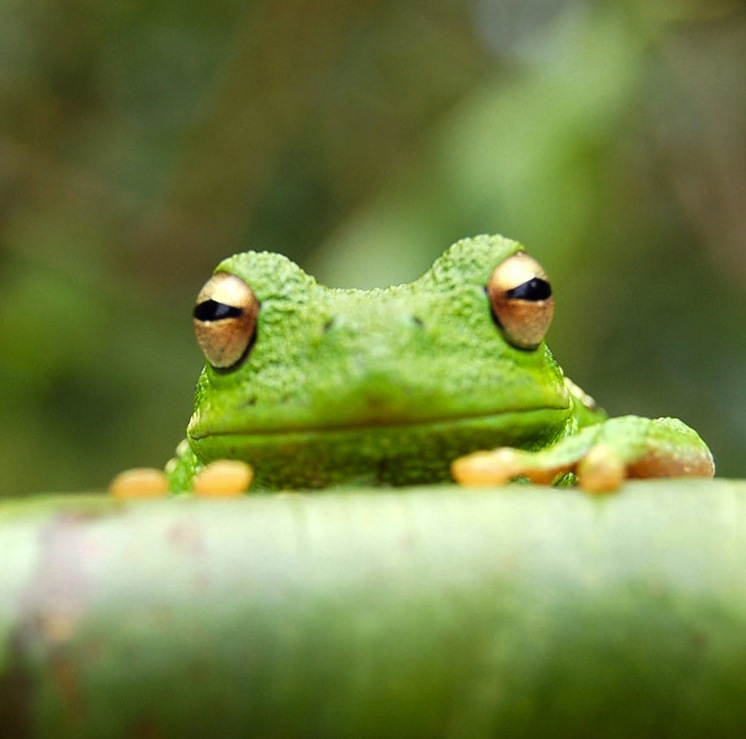
\includegraphics[width=0.3\textwidth]{frog.jpg} %or 4in or 4cm or 4pt
	\caption{Ribbit.}
	\label{fig:frog}
\end{figure}

\begin{figure}[h!]
\centering
\begin{subfigure}{.5\columnwidth}
  \centering
  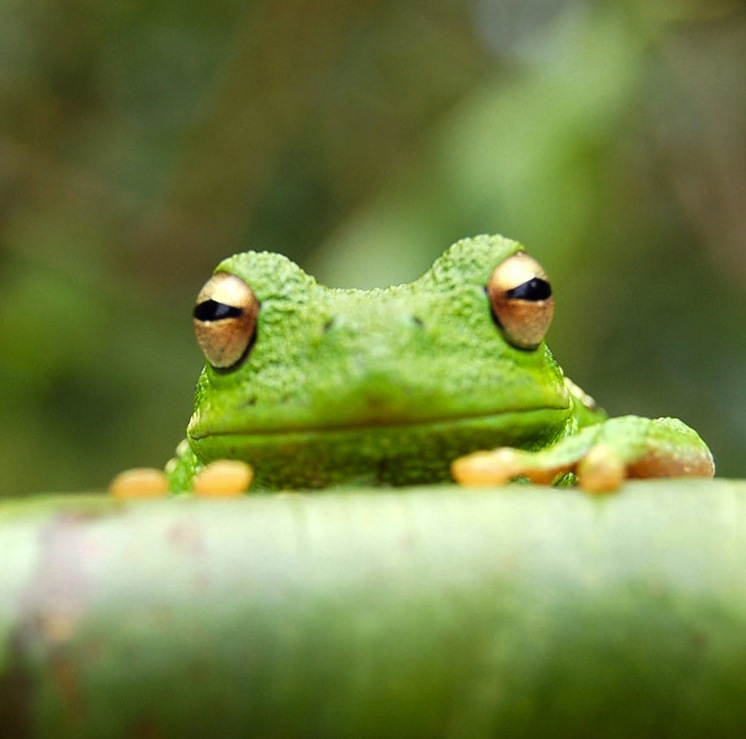
\includegraphics[width=2in]{frog.jpg} 
  \caption{A subfigure}
  \label{fig:sub1}
\end{subfigure}%
\begin{subfigure}{.5\columnwidth}
  \centering
  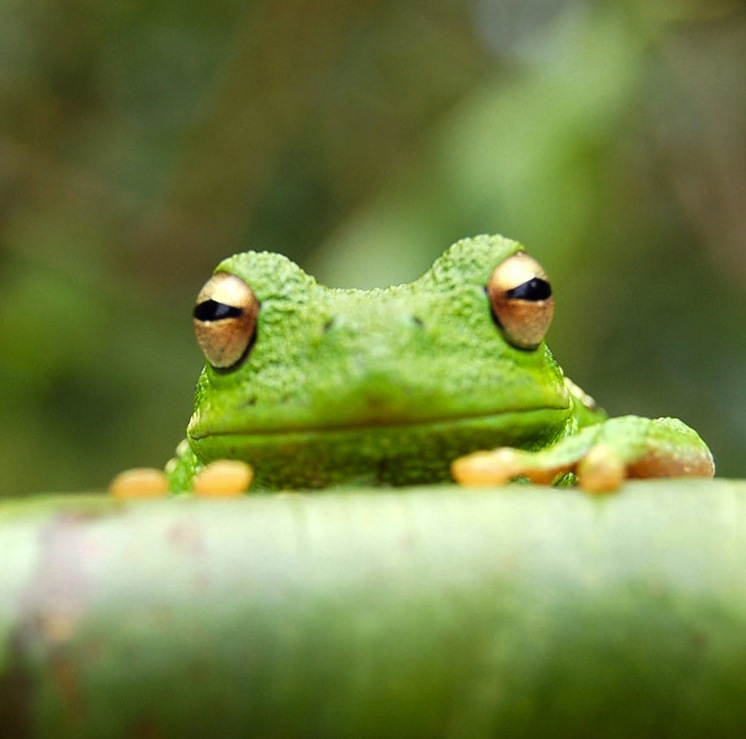
\includegraphics[width=.45\columnwidth]{frog.jpg}
  \caption{A subfigure}
  \label{fig:sub2}
\end{subfigure}
\caption{A figure with two subfigures that are sized using inches and \texttt{columnwidth}}
\label{fig:sidebyside}
\end{figure}


\subsection{How to Make Tables}

Use the table and tabular commands for basic tables --- see Table \ref{tab:widgets}, for example. The portion in the square brackets denotes where the table should be placed. The portion in the curly braces denotes how many columns there will be and their justification (left, right, center). You don't specify the number of rows and each column is broken up by \& signs and each new row is started with \verb!\\!. \verb!\hline! is used for horizontal lines. 

\begin{table}
	\centering
	\begin{tabular}[h]{l | c c c}
		Item & Quantity & & 2$\sigma$
		\\ \hline
		Widgets & 42 & $\pm$ & 5\\
		Gadgets & 13 & $\pm$ & 2
	\end{tabular}
	\caption{An example table.}
    \label{tab:widgets}
\end{table}

\subsection{How to Write Mathematics}

$\LaTeX$ is great at typesetting mathematics. Let $X_1, X_2, \ldots, X_n$ be a sequence of independent and identically distributed random variables with $\text{E}[X_i] = \mu$ and $\text{Var}[X_i] = \sigma^2 < \infty$, and let
$$S_n = \frac{X_1 + X_2 + \cdots + X_n}{n} %\frac is the fraction command
      = \frac{1}{n}\sum_{i}^{n} X_i$$
denote their mean. Then as $n$ approaches infinity, the random variables $\sqrt{n}(S_n - \mu)$ converge in distribution to a normal $\mathcal{N}(0, \sigma^2)$. \\

An example of multiline equations is shown in equation \ref{eqn:linear}

\begin{align} \label{eqn:linear} % remove the * to have the equations numbered
	2x & = 3y + 2z\\
	6y & = 3y - 8z + 2\sigma^2\\
	\Aboxed{85 & \quad \text{units}} \nonumber %or use \textrm for roman font, \boxed if you don't have an &
\end{align}



\subsection{How to Make Sections and Subsections}

Use section and subsection commands to organize your document. \LaTeX{} handles all the formatting and numbering automatically. Use ref and label commands for cross-references.

\subsection{How to Make Lists}

You can make lists with automatic numbering \dots

\begin{enumerate}
	\item Like this using the \texttt{enumerate} environment,
	\item and like this.
\end{enumerate}
\dots or bullet points using the \texttt{itemize} environment \dots
\begin{itemize}
	\item Like this,
	\item and like this.
\end{itemize}


\subsection{Spacing in $\LaTeX$}
$\LaTeX$ automatically handles spacing, so no matter how many spaces         I put between words (there are 5 spaces between "spaces" and "I" in the code), it all counts as a single space. To take control of spacing, using the \texttt{verbatim} environment.

\begin{verbatim}
See now all my                 spaces             are rendered!
\end{verbatim}

Spacing in when typesetting math is a little tricker, because it still only does one space but they're closer together, so you can use the \verb!~!, \verb!\quad! or \verb!\qquad! command to put in spaces (that's in order of less to more spaces).

\begin{align}
	\frac{n_{i+1}n_e}{n_i} &=\frac{2}{\Lambda^3} \quad \text{here the spacing is rendered}\\
	\frac{n_{i+1}n_e}{n_i} &=\frac{2}{\Lambda^3} \text{here it isn't}
\end{align}


\end{document} % You always need an end{document}